% =========================================================================
% Theater-level training study: figures, tables, and body text.
% Generated artifacts referenced here:
%   final_plots/training_curves_grid.pdf      (Fig: training curves, panels a-f)
%   final_plots/eval_theater_{overall,palisades,pyrenees,salamis}.pdf
%   final_plots/eval_theater_stats.csv        (all 40 pairwise tests)
% Regeneration: scripts/plot_training_curves.py, scripts/plot_eval_boxplots.py
% (invocations in session log), scripts/eval_stats_tables.py.
% Preamble requirements: \usepackage{graphicx}, \usepackage{subcaption},
% \usepackage{booktabs}
% All p-values in text and tables are PAIRED tests on seed-matched fires,
% Holm-corrected within each evaluation across all ten pairwise comparisons.
% =========================================================================

% ------------------------------------------------------------------ Fig. 4
\begin{figure*}[t]
  \centering
  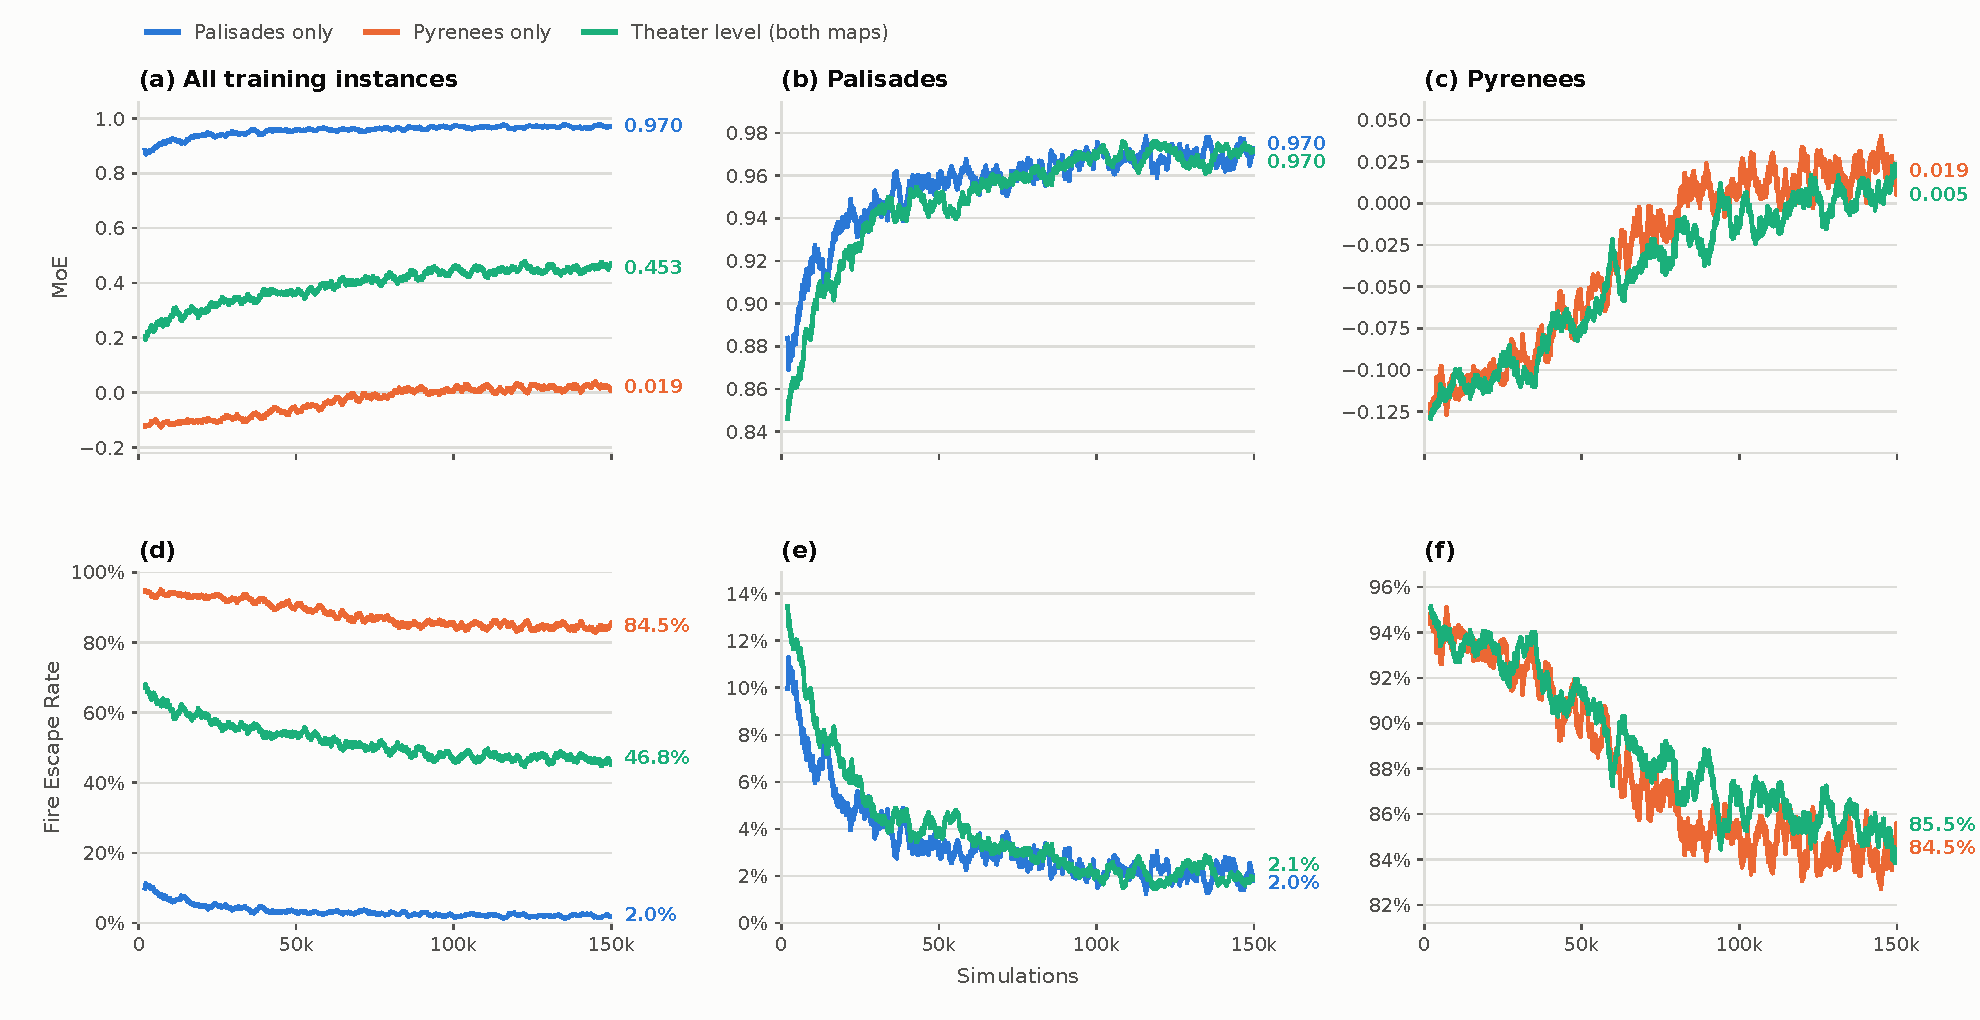
\includegraphics[width=\textwidth]{final_plots/training_curves_grid.pdf}
  \caption{Training dynamics of dedicated and theater-level mission
    coordination agents under a matched budget of 150{,}000 simulations.
    (a)~2{,}000-point moving average of MoE for all three training instances;
    MoE of the dedicated agent versus the theater-level agent's episodes on
    (b)~Palisades and (c)~Pyrenees; (d)--(f)~the corresponding fire escape
    rates. Curve-end labels report means over the final 20{,}000 simulations;
    panels (b), (c), (e), and (f) are magnified to the compared range.}
  \label{fig:theater-training}
\end{figure*}

In this section, we examine how the scope of the training theater shapes the
intelligent mission coordinator's performance.
Fig.~\ref{fig:theater-training} compares three training instances under an
identical budget of 150{,}000 simulations: an agent trained solely on
Palisades (blue), an agent trained solely on Pyrenees (orange), and a
theater-level agent trained on both scenarios concurrently (green) --- in
which each episode is randomly assigned to one of the two maps, so that a
single policy must serve the entire theater. Of the theater-level agent's
150{,}000 episodes, 65{,}569 were fought on Palisades and 84{,}431 on
Pyrenees. The x-axis represents the simulations and the y-axis represents the
MoE in the upper row (Fig.~\ref{fig:theater-training}.a--c) and the fire
escape rate --- the fraction of episodes in which the fire breaches
containment --- in the lower row (Fig.~\ref{fig:theater-training}.d--f). A
moving average of 2{,}000 simulations is utilized to smooth the training
noise, and the label at each curve end reports the mean over that instance's
final 20{,}000 simulations.

Fig.~\ref{fig:theater-training}.a and \ref{fig:theater-training}.d present
all three instances on common scales and establish the difficulty gap between
the two maps. On Palisades, the dedicated agent drives the escape rate from
roughly 11\% to 2.0\% while building its MoE from 0.87 to 0.970 by
interacting with the environment over time; on Pyrenees, escapes decline only
from 94\% to 84.5\%, with MoE climbing from $-0.13$ to 0.019. The
theater-level aggregate (mean MoE 0.453, escape rate 46.8\%) lies between the
two by construction, as it blends episodes from both maps, and is therefore
not directly comparable to either dedicated agent. We also note that the two
rows are near mirror images of one another; because the escape indicator
dominates the episode return, the MoE largely restates the escape rate rather
than capturing an independent dimension of performance.

Fig.~\ref{fig:theater-training}.b and \ref{fig:theater-training}.e compare
the Palisades-only agent against the theater-level agent's Palisades
episodes, drawn at the global simulation index so that the comparison
reflects equal computational budgets. Although the theater-level agent lags
over roughly the first 40{,}000 simulations --- its Palisades experience
accrues at less than half the dedicated rate --- it converges to a
statistically indistinguishable endpoint (MoE 0.970 versus 0.970; escape rate
2.1\% versus 2.0\%) despite encountering only 65{,}569 Palisades episodes
against the dedicated agent's 150{,}000. This suggests that theater-level
training is essentially free on the easier map: the concurrent agent recovers
full Palisades competence from 44\% of the data.

Fig.~\ref{fig:theater-training}.c and \ref{fig:theater-training}.f present
the corresponding comparison for Pyrenees, where the diverted budget carries
a small cost during training: the dedicated agent finishes 1.0 percentage
point ahead in escape rate (84.5\% versus 85.5\%, $p = 0.014$) and marginally
ahead in MoE (0.019 versus 0.005), with the two curves interleaving
throughout, indicating that the advantage is modest relative to the
simulation's inherent stochasticity. The persistence of high escape rates for
both agents underscores the environmental difficulty of Pyrenees, which
limits the achievable mission effectiveness regardless of the training
regime.

% ------------------------------------------------------------------ Fig. 5
\begin{figure*}[t]
  \centering
  \begin{subfigure}[t]{0.49\textwidth}
    \centering
    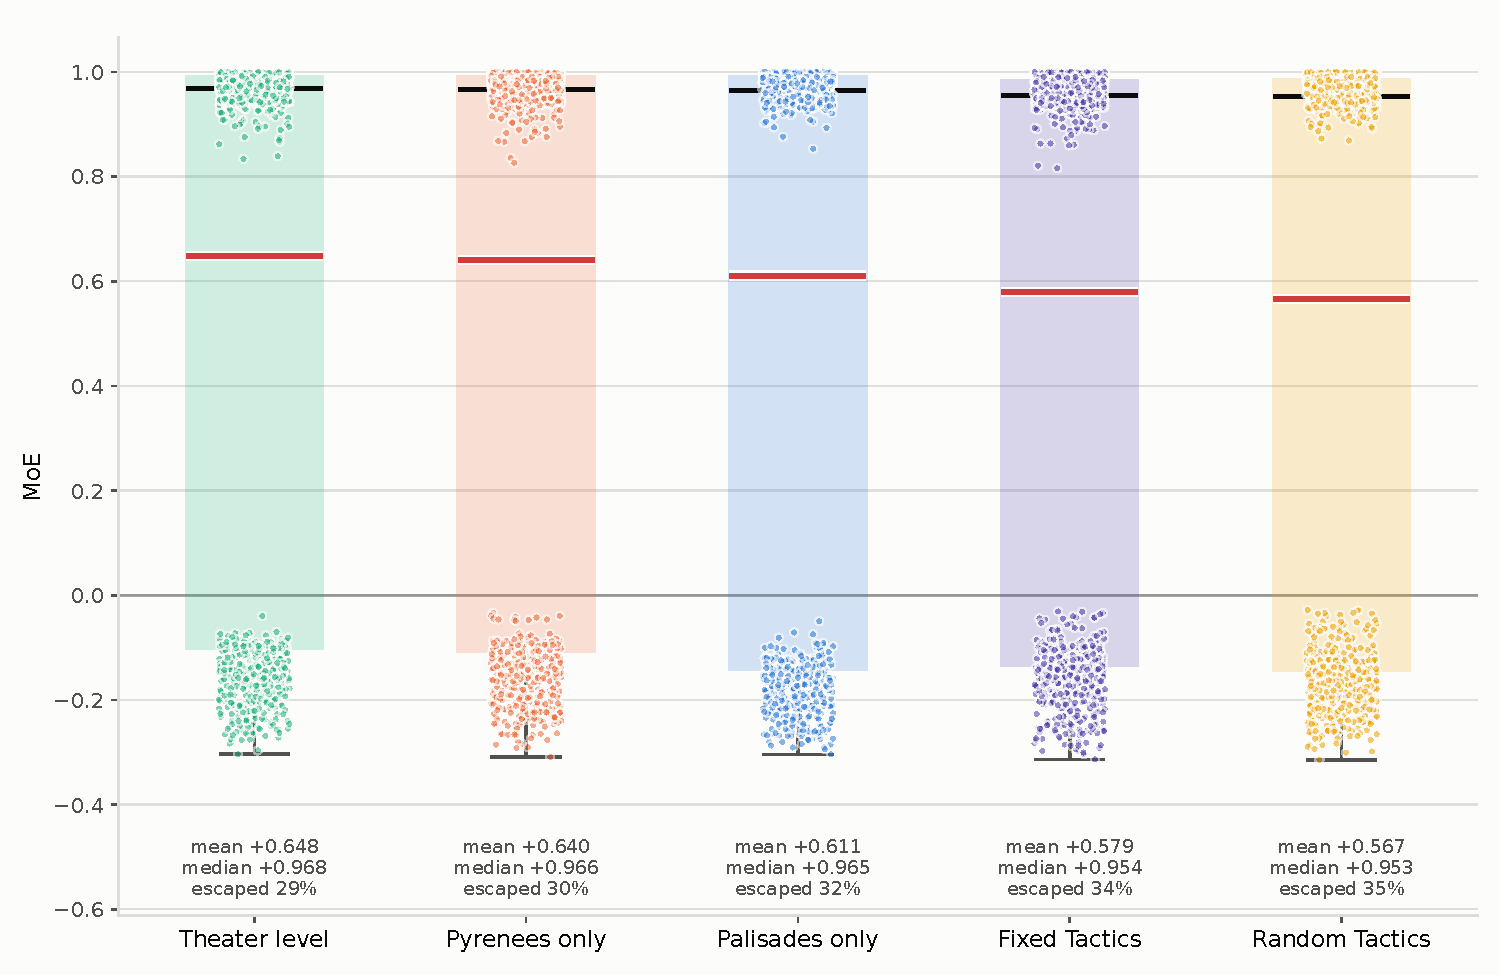
\includegraphics[width=\linewidth]{final_plots/eval_theater_overall.pdf}
    \caption{Overall, pooled across the three maps}
    \label{fig:eval-overall-panel}
  \end{subfigure}\hfill
  \begin{subfigure}[t]{0.49\textwidth}
    \centering
    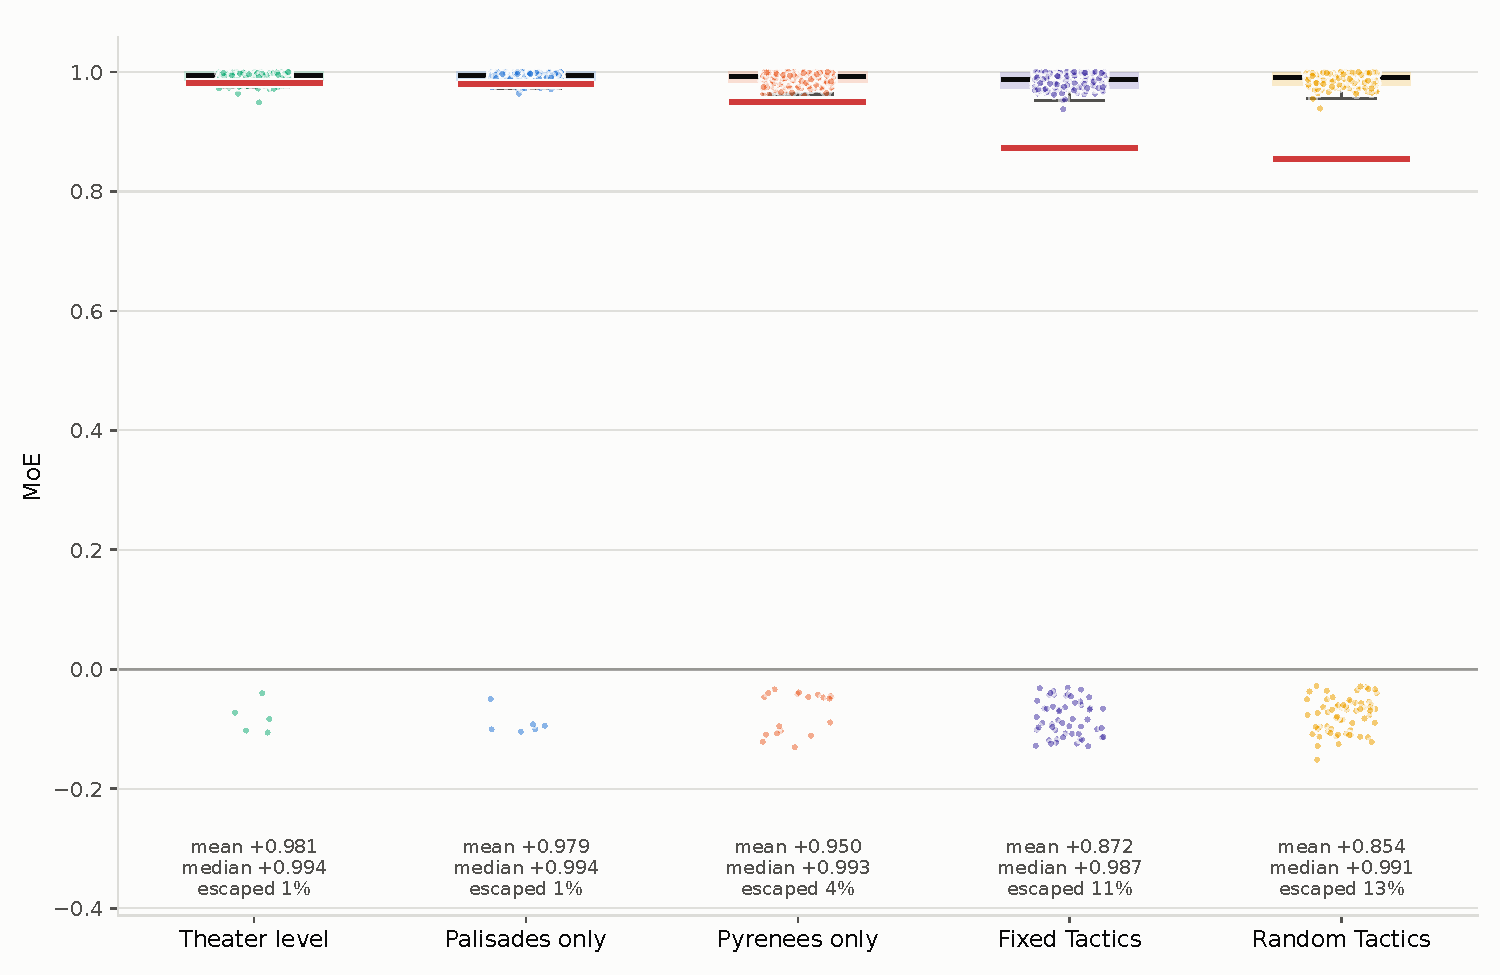
\includegraphics[width=\linewidth]{final_plots/eval_theater_palisades.pdf}
    \caption{Palisades}
    \label{fig:eval-palisades-panel}
  \end{subfigure}

  \vspace{4pt}

  \begin{subfigure}[t]{0.49\textwidth}
    \centering
    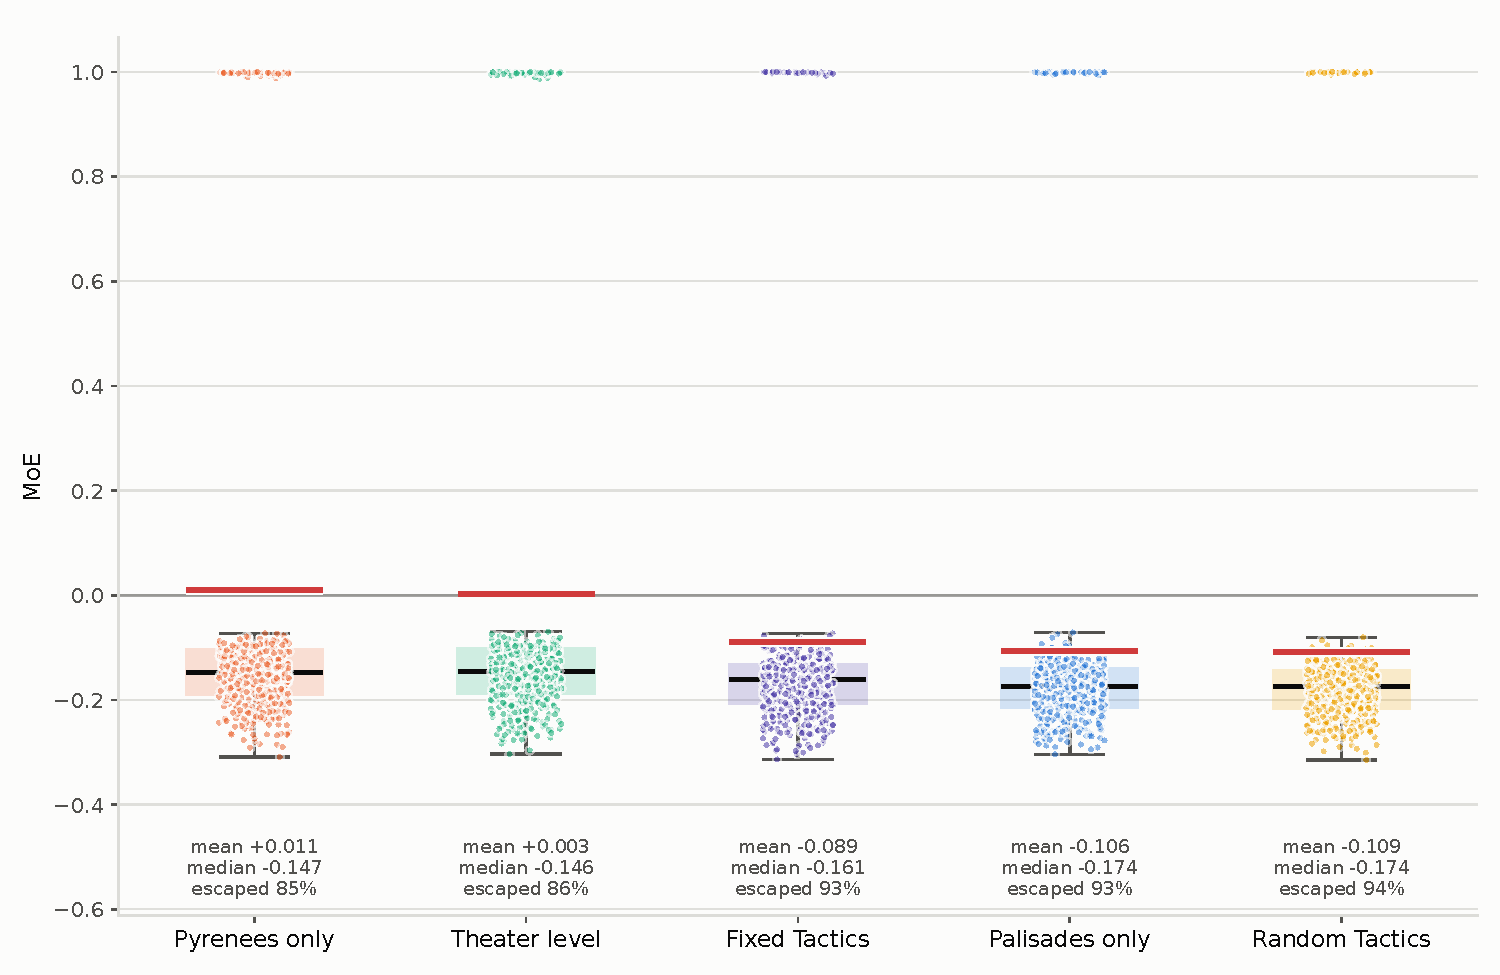
\includegraphics[width=\linewidth]{final_plots/eval_theater_pyrenees.pdf}
    \caption{Pyrenees}
    \label{fig:eval-pyrenees-panel}
  \end{subfigure}\hfill
  \begin{subfigure}[t]{0.49\textwidth}
    \centering
    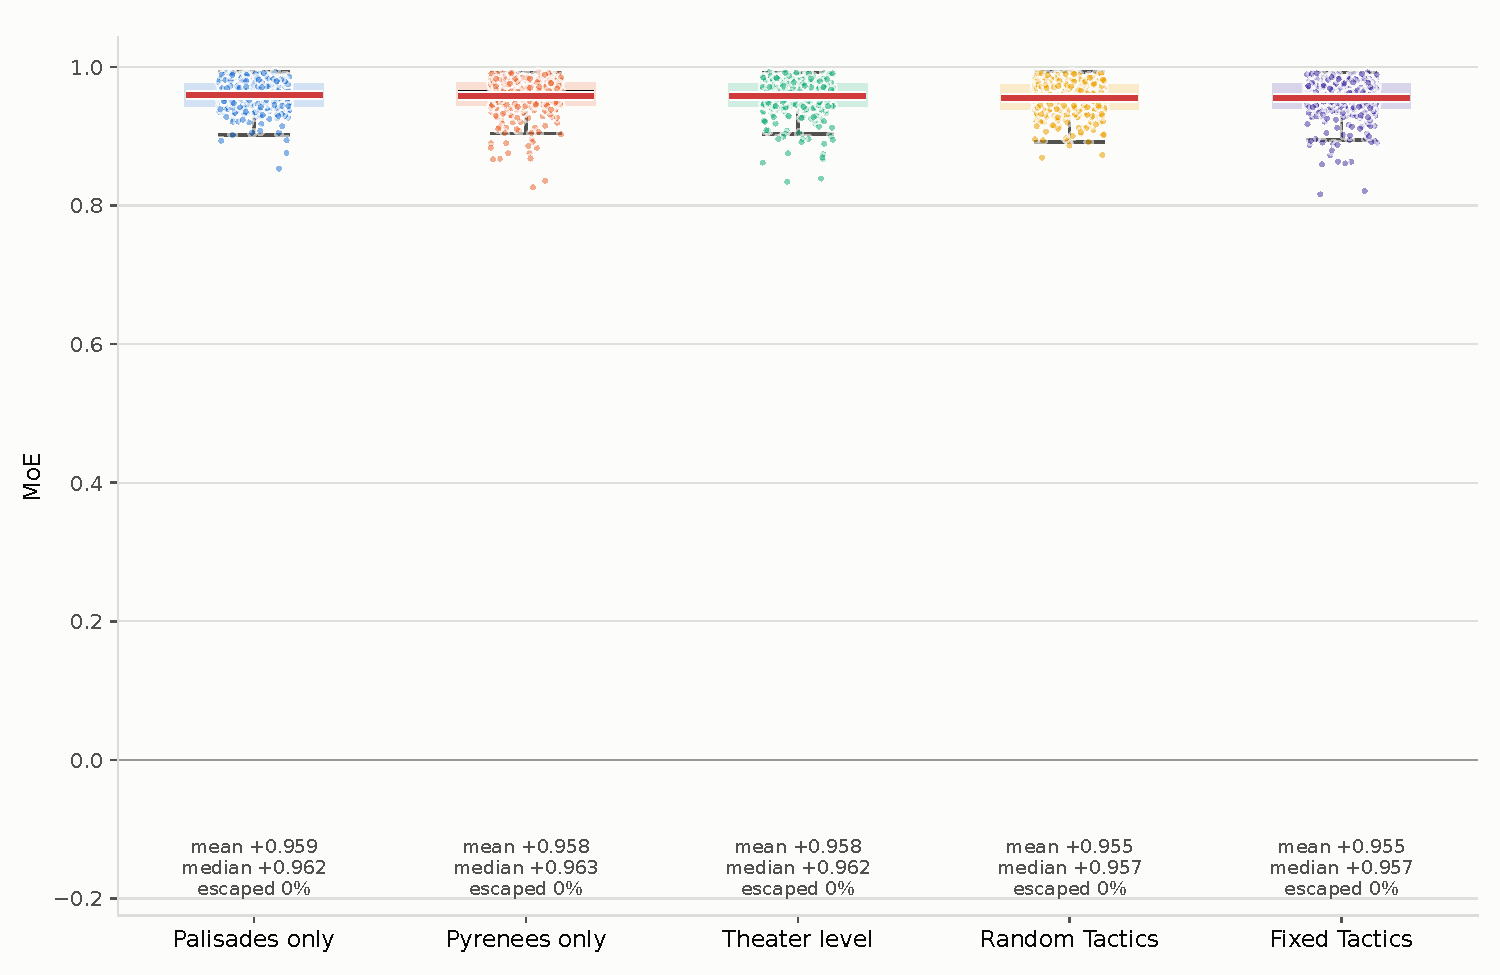
\includegraphics[width=\linewidth]{final_plots/eval_theater_salamis.pdf}
    \caption{Salamis, unseen in training}
    \label{fig:eval-salamis-panel}
  \end{subfigure}

  \caption{End-of-mission MoE of the three training instances --- Palisades-only
    (blue), Pyrenees-only (orange), and theater-level (green) --- against the
    Random Tactics (yellow) and Fixed Tactics (violet) baselines, over 500
    held-out ignitions per map, paired across policies by ignition seed. Each
    box spans the interquartile range, the black bar marks the median, the red
    line marks the mean, and the overlaid points show every individual
    simulation; the mean, median, and escape percentage are printed beneath
    each box. Within every panel, boxes are ordered left to right by decreasing
    mean MoE, while each policy keeps its color across panels. The evaluated
    models are the ${\sim}$100{,}000-simulation checkpoints of each instance.}
  \label{fig:eval-boxplots}
\end{figure*}

To assess the trained coordinators beyond their learning curves, we evaluate
the three training instances of Fig.~\ref{fig:theater-training} together with
two non-learned baselines: Random Tactics, in which a new tactic is randomly
assigned to each asset group every 10 minutes, and Fixed Tactics, a heuristic
containment configuration held constant throughout the mission.
Fig.~\ref{fig:eval-boxplots} presents the resulting MoE distributions, and
Tables~\ref{tab:eval-overall}--\ref{tab:eval-salamis} report the paired
statistics against the Random Tactics baseline. Because the MoE is nearly
binary --- a contained fire scores close to $+1$ and an escaped fire close to
$-0.15$ --- each distribution splits into two clusters, and the individual
simulation points are drawn over the boxes deliberately, as a box alone would
place its median in a gap where almost no simulation actually lands.

Fig.~\ref{fig:eval-overall-panel} and Table~\ref{tab:eval-overall} pool the
1{,}500 simulations per policy over Palisades, Pyrenees, and Salamis with
equal weight. Under this pooled view the theater-level agent ranks first with
a mean MoE of 0.648 (29\% escapes, $+0.081$ over Random Tactics,
$p < 0.001$), followed by Pyrenees-only (0.640), Palisades-only (0.611),
Fixed Tactics (0.579), and Random Tactics (0.567, 35\% escapes); the
theater-level agent's margin over the Pyrenees-only specialist, however, is
not itself significant ($p = 0.183$). Notably, Fixed Tactics does not
separate from Random Tactics on any evaluation ($p \geq 0.149$ throughout),
quantifying our earlier observation that random coordination is a strong
baseline in this environment.

Fig.~\ref{fig:eval-palisades-panel} and Table~\ref{tab:eval-palisades}
restrict the comparison to the 500 Palisades ignitions, where the separation
between learned and non-learned coordination is widest. The theater-level
agent attains the highest mean MoE of 0.981 with only 1\% of fires escaping,
statistically indistinguishable from the Palisades-only specialist at 0.979
($p = 0.76$); training on the full theater therefore costs nothing on this
map, consistent with the training curves. The Pyrenees-only agent transfers
imperfectly (0.950, 4\% escapes, $p = 0.011$ against the theater agent),
while both baselines trail by more than 0.10 MoE ($p < 0.001$). The point
clusters make the mechanism visible: all five policies contain the typical
Palisades fire with near-perfect MoE, and the ranking is driven almost
entirely by how often each policy lets a fire escape, which the learned
coordinators reduce by an order of magnitude relative to the baselines.

Fig.~\ref{fig:eval-pyrenees-panel} and Table~\ref{tab:eval-pyrenees} present
the same comparison on Pyrenees, the most demanding environment in the study.
Here the two clusters invert: the boxes of all five policies sit in the
failure cluster near $-0.15$, and the successful containments appear as the
sparse point cloud at $+1$. The Pyrenees-only specialist leads with a mean
MoE of 0.011 (85\% escapes), with the theater-level agent statistically
indistinguishable at 0.003 (86\% escapes, $p = 0.57$ before and $p = 1.0$
after Holm correction); the diverted training budget therefore costs the
theater agent no measurable evaluation performance on its harder map. Both
significantly outperform Fixed Tactics ($-0.089$), Random Tactics
($-0.109$), and, notably, the Palisades-only specialist ($-0.106$), which is
statistically indistinguishable from Random Tactics here ($p = 1.0$):
training on one map confers no advantage on the other, whereas the
theater-level agent retains specialist-level competence on both. Even the
best coordinators fail on the large majority of Pyrenees ignitions, so the
practical value of learned coordination on this map lies in roughly halving
the failure margin rather than eliminating it.

Fig.~\ref{fig:eval-salamis-panel} and Table~\ref{tab:eval-salamis} evaluate
all five policies on Salamis, a map that none of the learned agents
encountered during training. Every policy contains every fire --- no
simulation in any arm ends in an escape --- and the five means fall within
0.005 of one another. Under paired testing several of these tiny gaps
nevertheless reach statistical significance (the three learned agents exceed
Random Tactics by 0.003--0.004 MoE, $p < 0.001$), but no policy differs in
containment (McNemar $p = 1.0$ throughout), so the differences, while
detectable, are operationally negligible. This panel serves as a control:
Salamis is insensitive to tactical variance, so even random coordination
succeeds, and the figure demonstrates both that the learned policies transfer
to an unseen scenario without degradation and that outperforming on such a
scenario is not possible in any meaningful sense. The three-map evaluation
thus brackets the coordination problem --- a map where learning is decisive,
a map where it helps but cannot overcome the environment, and a map where it
is unnecessary --- and across all three, the theater-level agent is never
worse than the relevant specialist.

% ----------------------------------------------------------------- Tables
\begin{table}[t]
  \centering
  \caption{Paired evaluation statistics, overall (pooled across the three
    maps, 1{,}500 paired ignitions per policy). $\Delta$MoE is the policy's
    mean paired MoE difference against the Random Tactics baseline; $p_t$ is
    the paired $t$-test and $p_{\mathrm{McN}}$ the exact McNemar test on
    containment, both Holm-corrected within this evaluation across all ten
    pairwise comparisons.}
  \label{tab:eval-overall}
  \begin{tabular}{lrrrrr}
    \toprule
    Policy & Mean MoE & Escaped & $\Delta$MoE & $p_t$ & $p_{\mathrm{McN}}$ \\
    \midrule
    Theater level & $+0.648$ & 29\% & $+0.081$ & $<\!0.001$ & $<\!0.001$ \\
    Pyrenees only & $+0.640$ & 30\% & $+0.073$ & $<\!0.001$ & $<\!0.001$ \\
    Palisades only & $+0.611$ & 32\% & $+0.044$ & $<\!0.001$ & $<\!0.001$ \\
    Fixed Tactics & $+0.579$ & 34\% & $+0.013$ & $0.149$ & $0.292$ \\
    Random Tactics & $+0.567$ & 35\% & --- & --- & --- \\
    \bottomrule
  \end{tabular}
\end{table}

\begin{table}[t]
  \centering
  \caption{Paired evaluation statistics, Palisades (500 paired ignitions per
    policy). Columns as in Table~\ref{tab:eval-overall}.}
  \label{tab:eval-palisades}
  \begin{tabular}{lrrrrr}
    \toprule
    Policy & Mean MoE & Escaped & $\Delta$MoE & $p_t$ & $p_{\mathrm{McN}}$ \\
    \midrule
    Theater level & $+0.981$ & 1\% & $+0.128$ & $<\!0.001$ & $<\!0.001$ \\
    Palisades only & $+0.979$ & 1\% & $+0.126$ & $<\!0.001$ & $<\!0.001$ \\
    Pyrenees only & $+0.950$ & 4\% & $+0.097$ & $<\!0.001$ & $<\!0.001$ \\
    Fixed Tactics & $+0.872$ & 11\% & $+0.018$ & $0.635$ & $0.591$ \\
    Random Tactics & $+0.854$ & 13\% & --- & --- & --- \\
    \bottomrule
  \end{tabular}
\end{table}

\begin{table}[t]
  \centering
  \caption{Paired evaluation statistics, Pyrenees (500 paired ignitions per
    policy). Columns as in Table~\ref{tab:eval-overall}.}
  \label{tab:eval-pyrenees}
  \begin{tabular}{lrrrrr}
    \toprule
    Policy & Mean MoE & Escaped & $\Delta$MoE & $p_t$ & $p_{\mathrm{McN}}$ \\
    \midrule
    Pyrenees only & $+0.011$ & 85\% & $+0.120$ & $<\!0.001$ & $<\!0.001$ \\
    Theater level & $+0.003$ & 86\% & $+0.112$ & $<\!0.001$ & $<\!0.001$ \\
    Fixed Tactics & $-0.089$ & 93\% & $+0.020$ & $0.247$ & $1.000$ \\
    Palisades only & $-0.106$ & 93\% & $+0.002$ & $1.000$ & $1.000$ \\
    Random Tactics & $-0.109$ & 94\% & --- & --- & --- \\
    \bottomrule
  \end{tabular}
\end{table}

\begin{table}[t]
  \centering
  \caption{Paired evaluation statistics, Salamis (500 paired ignitions per
    policy). Columns as in Table~\ref{tab:eval-overall}.}
  \label{tab:eval-salamis}
  \begin{tabular}{lrrrrr}
    \toprule
    Policy & Mean MoE & Escaped & $\Delta$MoE & $p_t$ & $p_{\mathrm{McN}}$ \\
    \midrule
    Palisades only & $+0.959$ & 0\% & $+0.004$ & $<\!0.001$ & $1.000$ \\
    Pyrenees only & $+0.958$ & 0\% & $+0.003$ & $<\!0.001$ & $1.000$ \\
    Theater level & $+0.958$ & 0\% & $+0.003$ & $<\!0.001$ & $1.000$ \\
    Random Tactics & $+0.955$ & 0\% & --- & --- & --- \\
    Fixed Tactics & $+0.955$ & 0\% & $-0.000$ & $0.690$ & $1.000$ \\
    \bottomrule
  \end{tabular}
\end{table}
